\section{Theorie}
\label{sec:Theorie}
Alle Bilder und Informationen wurden aus dem Dokument \cite{v703} entnommen.
Das Geiger-Müller-Zählrohr wird in der Kernphysik verwendet, um die Intensität ionisierender Strahlung zu messen.
Dabei werden elektrische Impulse erzeugt, wenn $\alpha$- , $\beta$- oder $\gamma$- Teilchen absorbiert werden. In dem Versuch werden
einige Kenndaten eines Zählrohrs experimentell ermittelt.
\subsection{Aufbau und Funktionsweise}
Der schematische Aufbau eines Zählrohrs ist in Abbildung \ref{fig:aufbau} zu erkennen.
\begin{figure}
    \centering
    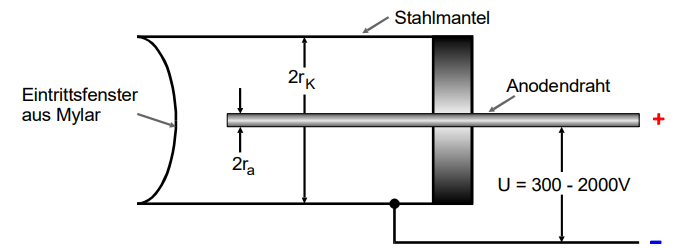
\includegraphics[scale=0.4]{pics/Aufbau.png}
    \caption{Querschnitt eines Endfenster-Zählrohrs}
    \label{fig:aufbau}
  \end{figure}
Es besteht aus einem Kathodenzylinder und einem darin axial verlaufenden Anodendraht. Im inneren befindet sich ein Gasgemisch.
Beim anlegen einer äußeren Spannung entsteht ein radialsymmetrisches Feld. Ein geladenes Teilchen, welches in das Zählrohrvolumen eindringt,
wird sich solange durch den Gasraum bewegen, bis seine Energie durch Ionisationsakte aufgebraucht ist. 
Es werden freie Elektronen und Ionen erzeugt. Die Anzahl der entstehenden Elektronen ist dabei Proportional zur Energie des einfallenden Teilchens.
\begin{figure}
    \centering
    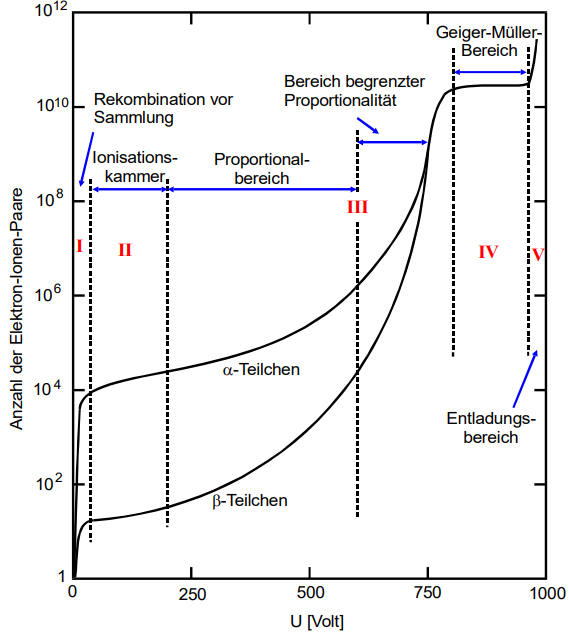
\includegraphics[scale=0.6]{pics/Elektronen.png}
    \caption{Detektierte Elektronen in Abhängigkeit von der Zählrohrspannung}
    \label{fig:Elektronen}
  \end{figure}
In Abbildung \ref{fig:Elektronen} ist erkennbar, dass die Anzahl der erzeugten Elektronen von der Zählrohrspannung $U$ abhängt.
Dabei werden fünf Bereiche unterschieden. Im ersten Bereich ist die angelegte Spannung nicht ausreichend, damit alle Elektronen den Draht erreichen, da viele 
durch Rekombination verloren gehen.
Bei ausreichender Spannung ist der Ionisationsstrom proportional zur Energie der einfallenden Strahlung.
Dieser Bereich wird als Ionisationskammer bezeichnet.
Jedoch kann diese Kammer praktisch nur für hohe Strahlintensitäten genutzt werden, da die Ströme sehr gering sind.
Der dritte Bereich wird als Proportionalitätsbereich bezeichnet. In diesem Bereich haben die 
Elektronen genügend Energie um durch Stoßionisation ihrerseits ionisieren zu können.
Die erzeugten freien Elektronen können ebenfalls ionisieren. Die Anzahl an freien Elektronen steigt damit lawinenartig an. Dieser Prozess wird als
Townsend-Lawine bezeichnet. Die gesammelte Ladung $Q$ ist Proportional zur Primärteilchenenergie. Somit lässt sich das Proportionalitätsrohr zur Energiemessung der
einfallenden Strahlung verwenden.
Bei weiterer Erhöhung der Betriebsspannung wird die Ladung $Q$ unabhängig von der Primärionisation. 
Die Ladung hängt nur noch vom Volumen und der Spannung ab. Dieser Effekt kommt durch die Entstehung von ungeladenen UV-Photonen, die sich auch Senkrecht zum E-Feld
ausbreiten können, wodurch weitere Lawinen im gesamten Zählrohrvolumen ausgelöst werden. 
Das Geiger-Müller-Zählrohr kann nur noch zur Intensitätsmessung benutzt werden.
Der lineare Anteil in diesem Bereich wird als Plateau bezeichnet. Dabei weisen hochwertigere Geiger-Müller-Zählrohre ein längeres und flacheres Plateau auf.
Wird die Spannung weiter erhöht, wird durch ein einzelnes Teilchen die Dauerentladung gezündet. Dies zerstört schnell das Zählrohr.
\subsection{Totzeit und Nachentladung}
Nach einer Entladung halten sich die positiven Ionen wegen ihrer größeren Masse länger als die Elektronen im Gasraum auf
und bilden eine vorübergehend radialsymmetrische, positive Raumladung.
Diese reduziert die effektive Feldstärke in Drahtnähe und verhindert somit die Stoßionisation für eine Zeit $\text{T}$.
Da in diesem Zeitraum keine weiteren Teilchen detektiert werden können, wird $\text{T}$ als Totzeit des Zählrohrs bezeichnet.
Nach der Totzeit wird ein weiterer Zeitraum $\text{T}_\text{E}$ zur vollständigen Neutralisation der Ionen benötigt.
Dieser Zeitraum wird Erholungszeit genannt, da der Entladungsimpuls erst nach dieser seine ursprüngliche Höhe erreicht.
Wie in Abbildung \ref{fig:tot} zu sehen, folgt die Erholungszeit auf die Totzeit.
\begin{figure}
  \centering
  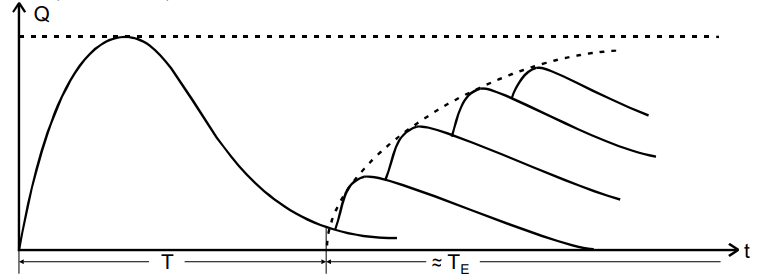
\includegraphics[scale=0.6]{pics/totzeit.png}
  \caption{Qualitative Darstellung der Tot- und Erholungszeit eines Zählrohrs}
  \label{fig:tot}
\end{figure}
Es ist möglich mit einem Oszilloskop die Kurve sichtbar zu machen, wodurch die Totzeit $\text{T}$ direkt ablesen werden kann.
Außerdem kann man mit der Zwei-Quellen-Methode die Totzeit $\text{T}$ bestimmen. 
Dabei werden bei zwei Präparaten, mit den Zählraten $N_1$ und $N_2$, die Zählraten einzeln und zusammen gemessen.
Die Totzeit berechnet sich dabei nach
\begin{equation}
  T_\text{T} \approx \frac{n_1 +n_2 -n_\text{1+2}}{2n_1 n_2} \, .
  \label{eqn:totzeit}
\end{equation}
Es kann zu sogenannten Nachentladungen während der Erholungszeit kommen. Diese entstehen dadurch, dass Ionen beim Neutralisieren am Zählrohrmantel
Elektronen herauslösen und somit neue Elektronenlawinen auslösen. Zur Reduzierung dieses Problems, kann dem Gas ein Alkoholzusatz beigemischt werden, welcher die 
Ionen im Gasraum neutralisiert. Die positiv geladenen Alkoholmoleküle bewegen sich anstelle der Ionen zum Zählrohrmantel. Diese können jedoch keine Elektronenlawinen mehr auslösen und werden am Zählrohrmantel neutralisiert.
Mit der Gleichung 
\begin{equation}
  Z=\frac{I}{e_0 N}
  \label{eqn:zstrom}
\end{equation}
lässt sich die Zahl der freigesetzten Ladungen pro einfallenen Teilchen berechnen. Dabei ist $I$ der mittlere Zählrohrstrom und $e_0$ die Elementarladung.
